\documentclass[conference]{IEEEtran}
\usepackage{amsmath,amssymb}
\usepackage{booktabs,float,graphicx,url}
\usepackage[hidelinks]{hyperref}
\graphicspath{{figures/}}
\setlength{\intextsep}{6pt plus 2pt minus 1pt}

\begin{document}
\title{Card Fraud Triage with Gaussian Mixtures and Deep Autoencoders}
\author{\IEEEauthorblockN{Palak Gupta \qquad Pratyush Parida}
\IEEEauthorblockA{Team ID T110}}
\maketitle
\raggedbottom

\begin{abstract}
Fraud triage requires rankings that surface rare frauds under limited review capacity. We compare a full-covariance Gaussian mixture model (GMM), a 12-dimensional autoencoder (AE), and a validation-selected blend on 56,962 chronologically held-out transactions containing 75 frauds. The base models are fitted on legitimate transactions. The AE uses deduplicated training features. The GMM achieves average precision of 0.4833 versus 0.2453 for the AE, while the AE leads in ROC-AUC (0.9274 versus 0.9106). Validation average precision selects a GMM weight of 1.00, so the blend reproduces the GMM ranking. At a validation false-positive budget of 0.10\%, the GMM detects 57 frauds with 35 false alerts, and the AE detects 22 with 30 false alerts. Every AE hit is also a GMM hit at that cutoff and in the first 100 reviews.
\end{abstract}

\begin{IEEEkeywords}
card fraud, anomaly detection, Gaussian mixture models, autoencoders, alert triage, average precision
\end{IEEEkeywords}

\section{Introduction and Operational Constraints}
The European card transaction benchmark contains 492 frauds among 284,807 transactions \cite{dalpozzolo}. Analysts can inspect only a fraction of alerts. A ranking can discriminate well over the full score range while returning too many false alerts near its head. We therefore report average precision (AP), ROC-AUC, recall and precision under fixed false-positive budgets, and precision and recall under fixed queue sizes. The held-out window contains 75 frauds, so one recovered fraud changes recall by about 1.33 percentage points.

\section{Related Work}
Dal Pozzolo \emph{et al.} \cite{dalpozzolo} use an imbalanced card dataset to study how undersampling changes the class prior and biases predicted probabilities. A prior correction can change calibration while preserving the ordering. We preserve the observed class proportions in validation and test and interpret detector outputs as anomaly scores. Dempster \emph{et al.} \cite{dempster} describe expectation-maximization (EM) for latent assignments, including finite mixtures. Sakurada and Yairi \cite{sakurada} compare nonlinear autoencoder reconstruction error against linear and kernel PCA on simulated dynamics and spacecraft telemetry. We apply reconstruction error to card transaction features and compare it with mixture likelihood under a review budget.

\section{Anti-Leakage Data Pipeline and Duplicate Audit}
A stable sort on elapsed \texttt{Time} precedes a chronological 60/20/20 split. Training uses only legitimate rows. We drop \texttt{Time} after splitting because elapsed time would expose a non-overlapping range at deployment. The 29 scoring features are the supplied PCA components V1--V28 and Amount. The Phase~1 scaler and GMM use the original 170,524 legitimate training rows. Phase~2 removes 5,245 repeated 29-feature vectors (3.076\%), leaving 165,279 rows for the AE and its scaler. Repeated feature vectors can overweight recurring patterns in the training loss. Validation (56,961 rows, 57 frauds) and test retain all arrivals.

In the 8-dimensional ablation, legitimate validation MSE decreased from 0.5953 to 0.5929 (Table~\ref{tab:ablation}). Each training partition has its own standardization, so the observed change reflects both altered sample weights and scaling. It is a single-run comparison, and validation AP in this ablation fell from 0.0745 to 0.0683.

\begin{table}[H]
\centering\footnotesize\setlength{\tabcolsep}{3pt}
\caption{Duplicate ablation (8D AE). The 99\% cutoff is derived from the respective legitimate training scores.}
\label{tab:ablation}
\begin{tabular}{@{}lrrrrr@{}}
\toprule
Train set & Train MSE & Val MSE & Cutoff & Val AP & Val ROC \\
\midrule
Full & .3471 & .5953 & 1.7199 & .0745 & .9445 \\
Dedup. & .3506 & .5929 & 1.7452 & .0683 & .9449 \\
\bottomrule
\end{tabular}
\end{table}


\begin{figure*}[!t]
\centering
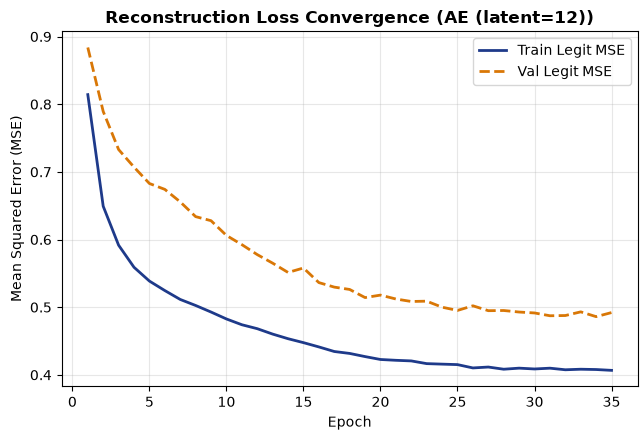
\includegraphics[width=0.37\textwidth]{ae_convergence.png}\hfill
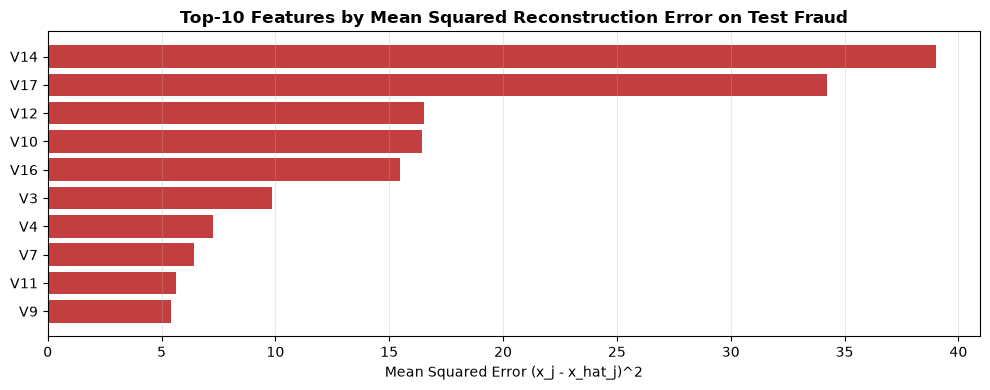
\includegraphics[width=0.60\textwidth]{ae_attribution.png}
\caption{Saved training-notebook outputs. Left, standard 12D AE loss by epoch. Right, the ten features with highest mean squared reconstruction error on test frauds.}
\label{fig:ae}
\end{figure*}

\section{Comparative Methodology}
\subsection{Full-covariance Gaussian mixture}
For standardized input $x\in\mathbb R^{D}$, $D=29$, the GMM is
\begin{align}
p(x)&=\sum_{k=1}^{K}\pi_k\mathcal N(x;\mu_k,\Sigma_k), \quad K=10,\\
\mathcal N(x;\mu,\Sigma)
&=\frac{\exp[-(x-\mu)^\top\Sigma^{-1}(x-\mu)/2]}
        {(2\pi)^{D/2}|\Sigma|^{1/2}},
\end{align}
where $\pi_k\ge0$ and $\sum_k\pi_k=1$. EM estimates latent responsibilities with the current parameters,
\begin{equation}
r_{ik}=\frac{\pi_k\mathcal N(x_i;\mu_k,\Sigma_k)}
{\sum_j\pi_j\mathcal N(x_i;\mu_j,\Sigma_j)}.
\end{equation}
For $N$ training rows, the update with covariance regularization is
\begin{align}
N_k &= \sum_i r_{ik}, \qquad \pi_k^{+}=N_k/N,\\
\mu_k^{+} &= N_k^{-1}\sum_i r_{ik}x_i,\\
\Sigma_k^{+} &= N_k^{-1}\sum_i r_{ik}(x_i-\mu_k^{+})
                     (x_i-\mu_k^{+})^\top + \lambda I .
\end{align}
The saved fit uses five initializations and $\lambda=10^{-6}$. Its score is $s_G(x)=-\log p(x)$.

\subsection{Nonlinear autoencoder}
The standard AE uses widths $29\to22\to14\to12\to14\to22\to29$. Hidden blocks use batch normalization and LeakyReLU (slope 0.1), with dropout of 0.10 after the first hidden block of each half. The bottleneck and reconstruction layers have linear outputs. For encoder $f_\theta$ and decoder $g_\phi$, training minimizes
\begin{equation}
\mathcal L(\theta,\phi)=\frac{1}{ND}\sum_{i=1}^N
\|x_i-g_\phi(f_\theta(\tilde x_i))\|_2^2 .
\end{equation}
For standard training, $\tilde x_i=x_i$. Denoising runs add independent Gaussian noise with standard deviation 0.05 in standardized input units. At inference, the clean standardized input gives the anomaly score
$s_A(x)=D^{-1}\|x-g_\phi(f_\theta(x))\|_2^2$.
We use the saved 12-dimensional standard AE, which led the sweep on validation AP. The sweep trained with AdamW and early stopping on legitimate validation MSE.

\subsection{Score fusion and triage}
We fit means $\mu_m$ and population standard deviations $\sigma_m$ on all validation scores for each detector $m$. The blend is
\begin{equation}
s_H(x)=\alpha\,\frac{s_G(x)-\mu_G}{\sigma_G}
+(1-\alpha)\,\frac{s_A(x)-\mu_A}{\sigma_A}.
\end{equation}
We select $\alpha$ by validation AP from $\{0,0.25,0.50,0.75,1\}$. The base fits use legitimate training data. Validation labels enter blend selection and identify legitimate validation rows for FPR calibration.

For target FPR $q$, sort the $N_0=56{,}904$ legitimate validation scores in descending order and flag scores strictly greater than the first excluded score, at rank $\lfloor q N_0\rfloor+1$. This limits validation false positives to $\lfloor q N_0\rfloor$ even with tied scores. We freeze the cutoff before scoring test. For fixed queues, we rank the test stream by descending score and use CSV order to break ties.

\begin{figure*}[!t]
\centering
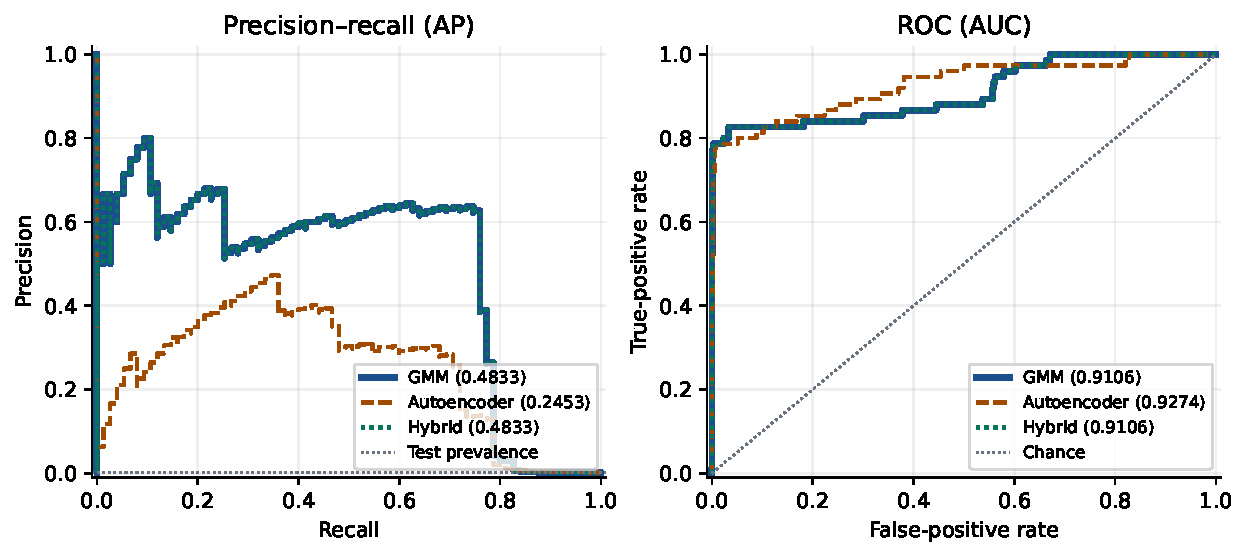
\includegraphics[width=0.97\textwidth]{test_curves.pdf}
\caption{Held-out precision--recall and ROC curves. The hybrid overlaps the GMM because the validation sweep selects $\alpha=1$. The PR reference is test fraud prevalence (75/56,962).}
\label{fig:curves}
\end{figure*}

\section{Unsupervised Manifold Evaluation and Triage Results}
Table~\ref{tab:sweep} compares bottlenecks and denoising variants. The 12-dimensional standard AE has the lowest legitimate validation MSE (0.4860) and highest validation AP (0.1222). The 16-dimensional model reconstructs the training sample more closely but gives higher validation MSE. Fig.~\ref{fig:ae} shows the original convergence and attribution plots. V14 and V17 exhibit fraud-to-legitimate mean squared reconstruction error ratios of 123.28 and 137.34 (Table~\ref{tab:attribution}). These PCA coordinates localize reconstruction error.
\begin{table}[H]
\centering\footnotesize\setlength{\tabcolsep}{3pt}
\caption{Bottleneck sweep. MSE uses legitimate rows. The 99\% cutoff uses the training split.}
\label{tab:sweep}
\resizebox{\columnwidth}{!}{%
\begin{tabular}{lrrrrrrrr}
\toprule
Model & $d$ & Noise & Params & Train MSE & Val MSE & Cutoff & Val AP & Val ROC \\
\midrule
AE & 4 & 0.00 & 2,253 & 0.4907 & 0.7418 & 2.3849 & 0.0478 & 0.9357 \\
AE & 8 & 0.00 & 2,369 & 0.3506 & 0.5929 & 1.7452 & 0.0683 & 0.9449 \\
AE & 12 & 0.00 & 2,485 & 0.2967 & 0.4860 & 1.4322 & 0.1222 & 0.9467 \\
AE & 16 & 0.00 & 2,601 & 0.2884 & 0.5121 & 1.5165 & 0.0785 & 0.9415 \\
DAE & 8 & 0.05 & 2,369 & 0.3654 & 0.6070 & 1.8661 & 0.0616 & 0.9369 \\
DAE & 12 & 0.05 & 2,485 & 0.3068 & 0.5405 & 1.4879 & 0.0846 & 0.9531 \\
\bottomrule
\end{tabular}}
\end{table}

\begin{table}[H]
\centering\footnotesize\setlength{\tabcolsep}{3pt}
\caption{Top ten features by mean squared error on test frauds.}
\label{tab:attribution}
\begin{tabular}{lrrr}
\toprule
Feature & Legit MSE & Fraud MSE & Fraud/legit \\
\midrule
V14 & 0.3164 & 38.9999 & 123.28 \\
V17 & 0.2494 & 34.2506 & 137.34 \\
V12 & 0.2763 & 16.5218 & 59.79 \\
V10 & 0.2267 & 16.4190 & 72.42 \\
V16 & 0.3648 & 15.4536 & 42.36 \\
V3 & 1.2007 & 9.8601 & 8.21 \\
V4 & 0.3461 & 7.2553 & 20.97 \\
V7 & 0.3577 & 6.4272 & 17.97 \\
V11 & 0.6946 & 5.6463 & 8.13 \\
V9 & 0.3259 & 5.4359 & 16.68 \\
\bottomrule
\end{tabular}
\end{table}


The geometry audit compares hard GMM assignments in standardized 29-dimensional space with 10-cluster $k$-means assignments in the 12-dimensional latent space. The metrics use a seeded sample of 10,000 test rows and no fraud labels. The latent representation gives higher Silhouette and Calinski--Harabasz and lower Davies--Bouldin values (Table~\ref{tab:geometry}). The clustering algorithm also changes, so the comparison does not isolate the effect of representation. The pseudo-label agreement experiment (Tables~\ref{tab:consensus} and~\ref{tab:pseudo}) applies training score quantiles to test. It is a distinct protocol from the validation false-positive budgets.
\begin{table}[H]
\centering\footnotesize\setlength{\tabcolsep}{3pt}
\caption{Intrinsic cluster metrics (10 clusters per space).}
\label{tab:geometry}
\begin{tabular}{@{}lrrr@{}}
\toprule
Space / assignments & Silhouette $\uparrow$ & DB $\downarrow$ & CH $\uparrow$ \\
\midrule
29D / GMM & 0.0364 & 4.4603 & 168.82 \\
12D / $k$-means & 0.1836 & 1.5472 & 1048.19 \\
\bottomrule
\end{tabular}
\end{table}

\begin{table}[H]
\centering\footnotesize\setlength{\tabcolsep}{3pt}
\caption{Training-quantile pseudo-label agreement. Cutoffs come from scores on deduplicated legitimate training rows. Alert counts and agreement use test.}
\label{tab:consensus}
\resizebox{\columnwidth}{!}{%
\begin{tabular}{lrrrrrrrr}
\toprule
Quantile & GMM cut & AE cut & GMM & AE & Both & $\kappa$ & Jaccard & Spear. $\rho$ \\
\midrule
99.0\% & 52.056 & 1.4322 & 880 & 854 & 495 & 0.5643 & 0.3995 & 0.5049 \\
99.5\% & 57.504 & 2.0401 & 530 & 397 & 283 & 0.6074 & 0.4394 & 0.5049 \\
99.9\% & 86.735 & 5.8213 & 120 & 88 & 72 & 0.6918 & 0.5294 & 0.5049 \\
\bottomrule
\end{tabular}}
\end{table}

\begin{table}[H]
\centering\footnotesize\setlength{\tabcolsep}{3pt}
\caption{Test audit of 99.9\% train-quantile pseudo-labels.}
\label{tab:pseudo}
\begin{tabular}{@{}lrrrrr@{}}
\toprule
Rule & Alerts & TP & FP & Prec. (\%) & Recall (\%) \\
\midrule
GMM & 120 & 57 & 63 & 47.50 & 76.00 \\
AE & 88 & 34 & 54 & 38.64 & 45.33 \\
Both & 72 & 34 & 38 & 47.22 & 45.33 \\
\bottomrule
\end{tabular}
\end{table}


Table~\ref{tab:blend} shows the validation sweep. At $\alpha=1$, the hybrid is the GMM score under positive affine rescaling, which leaves rankings and corresponding alert decisions unchanged. On test (Table~\ref{tab:ranking} and Fig.~\ref{fig:curves}), GMM leads on AP and AE leads on ROC-AUC. Phase~1 reported trapezoidal PR area of 0.4736 for GMM. Here we use scikit-learn's non-interpolated AP, which weights precision by increments in recall.
\begin{table}[H]
\centering\footnotesize\setlength{\tabcolsep}{3pt}
\caption{Blend selection on validation.}
\label{tab:blend}
\begin{tabular}{lrr}
\toprule
GMM weight $\alpha$ & AP & ROC-AUC \\
\midrule
0.00 & 0.1222 & 0.9467 \\
0.25 & 0.1550 & 0.9476 \\
0.50 & 0.1842 & 0.9458 \\
0.75 & 0.2437 & 0.9402 \\
1.00 & 0.4782 & 0.9351 \\
\bottomrule
\end{tabular}
\end{table}

\begin{table}[H]
\centering\footnotesize\setlength{\tabcolsep}{3pt}
\caption{Global ranking on the held-out test split.}
\label{tab:ranking}
\begin{tabular}{lrr}
\toprule
Model & AP & ROC-AUC \\
\midrule
GMM & 0.4833 & 0.9106 \\
AE & 0.2453 & 0.9274 \\
Hybrid & 0.4833 & 0.9106 \\
\bottomrule
\end{tabular}
\end{table}


Under the tightest validation FPR budget, GMM reaches 76.0\% recall and 61.96\% precision. AE reaches 29.33\% recall and 42.31\% precision. At the 0.50\% budget, the AE has higher precision and lower recall than GMM. Their realized test FPRs differ, so Table~\ref{tab:operating} includes both the target and realized rate. In equal-size queues, GMM leads at $K=50,100,200$ and ties the AE at $K=500$, where each retrieves 59 frauds (Table~\ref{tab:queues}).
\begin{table}[H]
\centering\footnotesize\setlength{\tabcolsep}{3pt}
\caption{Validation-only cutoffs and realized test triage. Each model flags 56, 284 and 569 legitimate validation rows at the respective budgets (0.0984\%, 0.4991\%, 0.9999\%).}
\label{tab:operating}
\resizebox{\columnwidth}{!}{%
\begin{tabular}{lrrrrrrr}
\toprule
Model & Val (\%) & Cutoff & TP & FP & FPR (\%) & Recall (\%) & Prec. (\%) \\
\midrule
GMM & 0.10 & 114.749583 & 57 & 35 & 0.0615 & 76.00 & 61.96 \\
GMM & 0.50 & 68.723566 & 59 & 192 & 0.3375 & 78.67 & 23.51 \\
GMM & 1.00 & 60.692267 & 59 & 346 & 0.6082 & 78.67 & 14.57 \\
AE & 0.10 & 9.780338 & 22 & 30 & 0.0527 & 29.33 & 42.31 \\
AE & 0.50 & 3.057487 & 53 & 141 & 0.2479 & 70.67 & 27.32 \\
AE & 1.00 & 2.016608 & 55 & 346 & 0.6082 & 73.33 & 13.72 \\
Hybrid & 0.10 & 0.983374 & 57 & 35 & 0.0615 & 76.00 & 61.96 \\
Hybrid & 0.50 & 0.665640 & 59 & 192 & 0.3375 & 78.67 & 23.51 \\
Hybrid & 1.00 & 0.610197 & 59 & 346 & 0.6082 & 78.67 & 14.57 \\
\bottomrule
\end{tabular}}
\end{table}

\begin{table}[H]
\centering\footnotesize\setlength{\tabcolsep}{3pt}
\caption{Fixed review queues. Cells show true positives and precision / recall in percent.}
\label{tab:queues}
\begin{tabular}{rrrr}
\toprule
$K$ & GMM & AE & Hybrid \\
\midrule
50 & 29; 58.0 / 38.7 & 20; 40.0 / 26.7 & 29; 58.0 / 38.7 \\
100 & 57; 57.0 / 76.0 & 35; 35.0 / 46.7 & 57; 57.0 / 76.0 \\
200 & 58; 29.0 / 77.3 & 53; 26.5 / 70.7 & 58; 29.0 / 77.3 \\
500 & 59; 11.8 / 78.7 & 59; 11.8 / 78.7 & 59; 11.8 / 78.7 \\
\bottomrule
\end{tabular}
\end{table}


\section{Error Analysis and Conclusion}
At the 0.10\% validation budget, the models catch 22 frauds in common and GMM catches 35 additional frauds. In Top~100 the counts are 35 and 22. Both rules miss the same 18 cases and neither produces an AE-only hit (Table~\ref{tab:overlap}). The GMM-only cases have more negative median V14, V17 and V12 than shared misses at both operating rules (Table~\ref{tab:profiles}). Median Amount for GMM-only hits is 10.70 at the cutoff and 7.13 in the queue, versus 7.80 for shared misses, with overlapping interquartile ranges. Table~\ref{tab:indices} lists the exact test row positions.
\begin{table}[H]
\centering\footnotesize\setlength{\tabcolsep}{3pt}
\caption{Fraud overlap by operating rule. Each row totals 75.}
\label{tab:overlap}
\begin{tabular}{@{}lrrrr@{}}
\toprule
Rule & Both & GMM only & AE only & Missed \\
\midrule
Val FPR 0.10\% & 22 & 35 & 0 & 18 \\
Top 100 & 35 & 22 & 0 & 18 \\
\bottomrule
\end{tabular}
\end{table}

\begin{table}[H]
\centering\footnotesize\setlength{\tabcolsep}{1.6pt}
\caption{Raw feature medians [Q1, Q3]. The percentage denotes the validation FPR budget. GMM and AE rows list exclusive hits.}
\label{tab:profiles}
\begin{tabular}{@{}llrcccc@{}}
\toprule
Rule & Group & $n$ & Amount & V14 & V17 & V12 \\
\midrule
0.10\% & Both & 22 & \shortstack{1.00\\{\scriptsize [0.77,3.79]}} & \shortstack{-11.93\\{\scriptsize [-13.15,-8.60]}} & \shortstack{-5.73\\{\scriptsize [-6.54,-3.52]}} & \shortstack{-6.40\\{\scriptsize [-7.93,-5.98]}} \\
0.10\% & GMM & 35 & \shortstack{10.70\\{\scriptsize [0.98,139.34]}} & \shortstack{-6.28\\{\scriptsize [-8.49,-4.84]}} & \shortstack{-2.52\\{\scriptsize [-4.31,-1.38]}} & \shortstack{-3.81\\{\scriptsize [-4.84,-3.05]}} \\
0.10\% & AE & 0 & --- & --- & --- & --- \\
0.10\% & Missed & 18 & \shortstack{7.80\\{\scriptsize [2.28,36.89]}} & \shortstack{-1.89\\{\scriptsize [-2.97,-0.46]}} & \shortstack{1.33\\{\scriptsize [0.41,2.24]}} & \shortstack{-0.17\\{\scriptsize [-0.50,0.47]}} \\
Top 100 & Both & 35 & \shortstack{1.00\\{\scriptsize [0.77,48.86]}} & \shortstack{-9.15\\{\scriptsize [-12.45,-6.77]}} & \shortstack{-5.13\\{\scriptsize [-6.23,-2.79]}} & \shortstack{-6.12\\{\scriptsize [-7.33,-5.36]}} \\
Top 100 & GMM & 22 & \shortstack{7.13\\{\scriptsize [0.98,71.26]}} & \shortstack{-5.94\\{\scriptsize [-8.42,-4.60]}} & \shortstack{-1.80\\{\scriptsize [-3.43,-0.96]}} & \shortstack{-3.12\\{\scriptsize [-3.96,-2.68]}} \\
Top 100 & AE & 0 & --- & --- & --- & --- \\
Top 100 & Missed & 18 & \shortstack{7.80\\{\scriptsize [2.28,36.89]}} & \shortstack{-1.89\\{\scriptsize [-2.97,-0.46]}} & \shortstack{1.33\\{\scriptsize [0.41,2.24]}} & \shortstack{-0.17\\{\scriptsize [-0.50,0.47]}} \\
\bottomrule
\end{tabular}
\end{table}


On this time window, GMM yielded the strongest short-queue ranking and the validation-selected blend added no AE weight. The AE representation showed stronger intrinsic cluster geometry and a higher ROC-AUC. The contrast illustrates why ranking and review-budget metrics are needed alongside geometry. These findings come from one benchmark, one saved fit per method, and 75 held-out frauds. Calibration limits false alerts in validation, and realized false-positive rates can shift in future time windows.

\appendix
\section*{Fraud Row Positions}
\begin{table}[H]
\centering\footnotesize\setlength{\tabcolsep}{2pt}
\caption{Zero-based fraud row positions in the held-out CSV. Empty groups are marked with a dash.}
\label{tab:indices}
\begin{tabular}{@{}p{.19\columnwidth}p{.77\columnwidth}@{}}
\toprule Group & Test row positions \\ \midrule
\multicolumn{2}{@{}l}{\textit{Validation FPR budget of 0.10\%}} \\
Both & 6729, 7771, 7789, 10377, 15548, 15702, 15854, 15904, 16003, 16159, 16488, 21983, 22118, 22916, 24059, 24279, 34715, 34981, 35429, 35479, 36032, 40530 \\
GMM only & 1867, 2231, 2631, 5413, 6787, 6788, 6860, 7799, 9262, 10521, 11654, 11656, 13409, 13600, 19828, 20150, 20451, 21126, 21322, 21762, 23632, 24021, 24929, 27558, 27711, 30558, 33211, 33628, 34080, 46630, 49019, 52018, 52298, 52304, 53299 \\
AE only & --- \\
Missed & 1885, 4133, 9581, 10621, 12377, 17502, 17711, 21394, 24036, 24046, 26499, 26550, 35235, 44676, 46537, 48147, 48226, 53829 \\
\midrule\multicolumn{2}{@{}l}{\textit{Top 100 queue}} \\
Both & 1867, 2231, 2631, 6729, 7771, 7789, 7799, 10377, 13600, 15548, 15702, 15854, 15904, 16003, 16159, 16488, 19828, 21322, 21762, 21983, 22118, 22916, 23632, 24021, 24059, 24279, 24929, 34715, 34981, 35429, 35479, 36032, 40530, 52018, 53299 \\
GMM only & 5413, 6787, 6788, 6860, 9262, 10521, 11654, 11656, 13409, 20150, 20451, 21126, 27558, 27711, 30558, 33211, 33628, 34080, 46630, 49019, 52298, 52304 \\
AE only & --- \\
Missed & Same 18 rows as the 0.10\% rule. \\
\bottomrule
\end{tabular}
\end{table}


\begin{thebibliography}{00}
\bibitem{dalpozzolo}
A. Dal Pozzolo, O. Caelen, R. A. Johnson, and G. Bontempi, \emph{Calibrating probability with undersampling for unbalanced classification}, in Proc. IEEE Symp. Series Comput. Intell., 2015, pp. 159--166. \href{https://www3.nd.edu/~dial/publications/dalpozzolo2015calibrating.pdf}{Paper}.
\bibitem{dempster}
A. P. Dempster, N. M. Laird, and D. B. Rubin, \emph{Maximum likelihood from incomplete data via the EM algorithm}, J. Roy. Stat. Soc. B, vol. 39, no. 1, pp. 1--38, 1977. \href{https://doi.org/10.1111/j.2517-6161.1977.tb01600.x}{DOI}.
\bibitem{sakurada}
M. Sakurada and T. Yairi, \emph{Anomaly detection using autoencoders with nonlinear dimensionality reduction}, in Proc. 2nd Workshop Mach. Learn. Sensory Data Anal., 2014, pp. 4--11. \href{https://doi.org/10.1145/2689746.2689747}{DOI}.
\end{thebibliography}
\end{document}
